\section{Setup}
\begin{figure}[htbp]
    \centering
    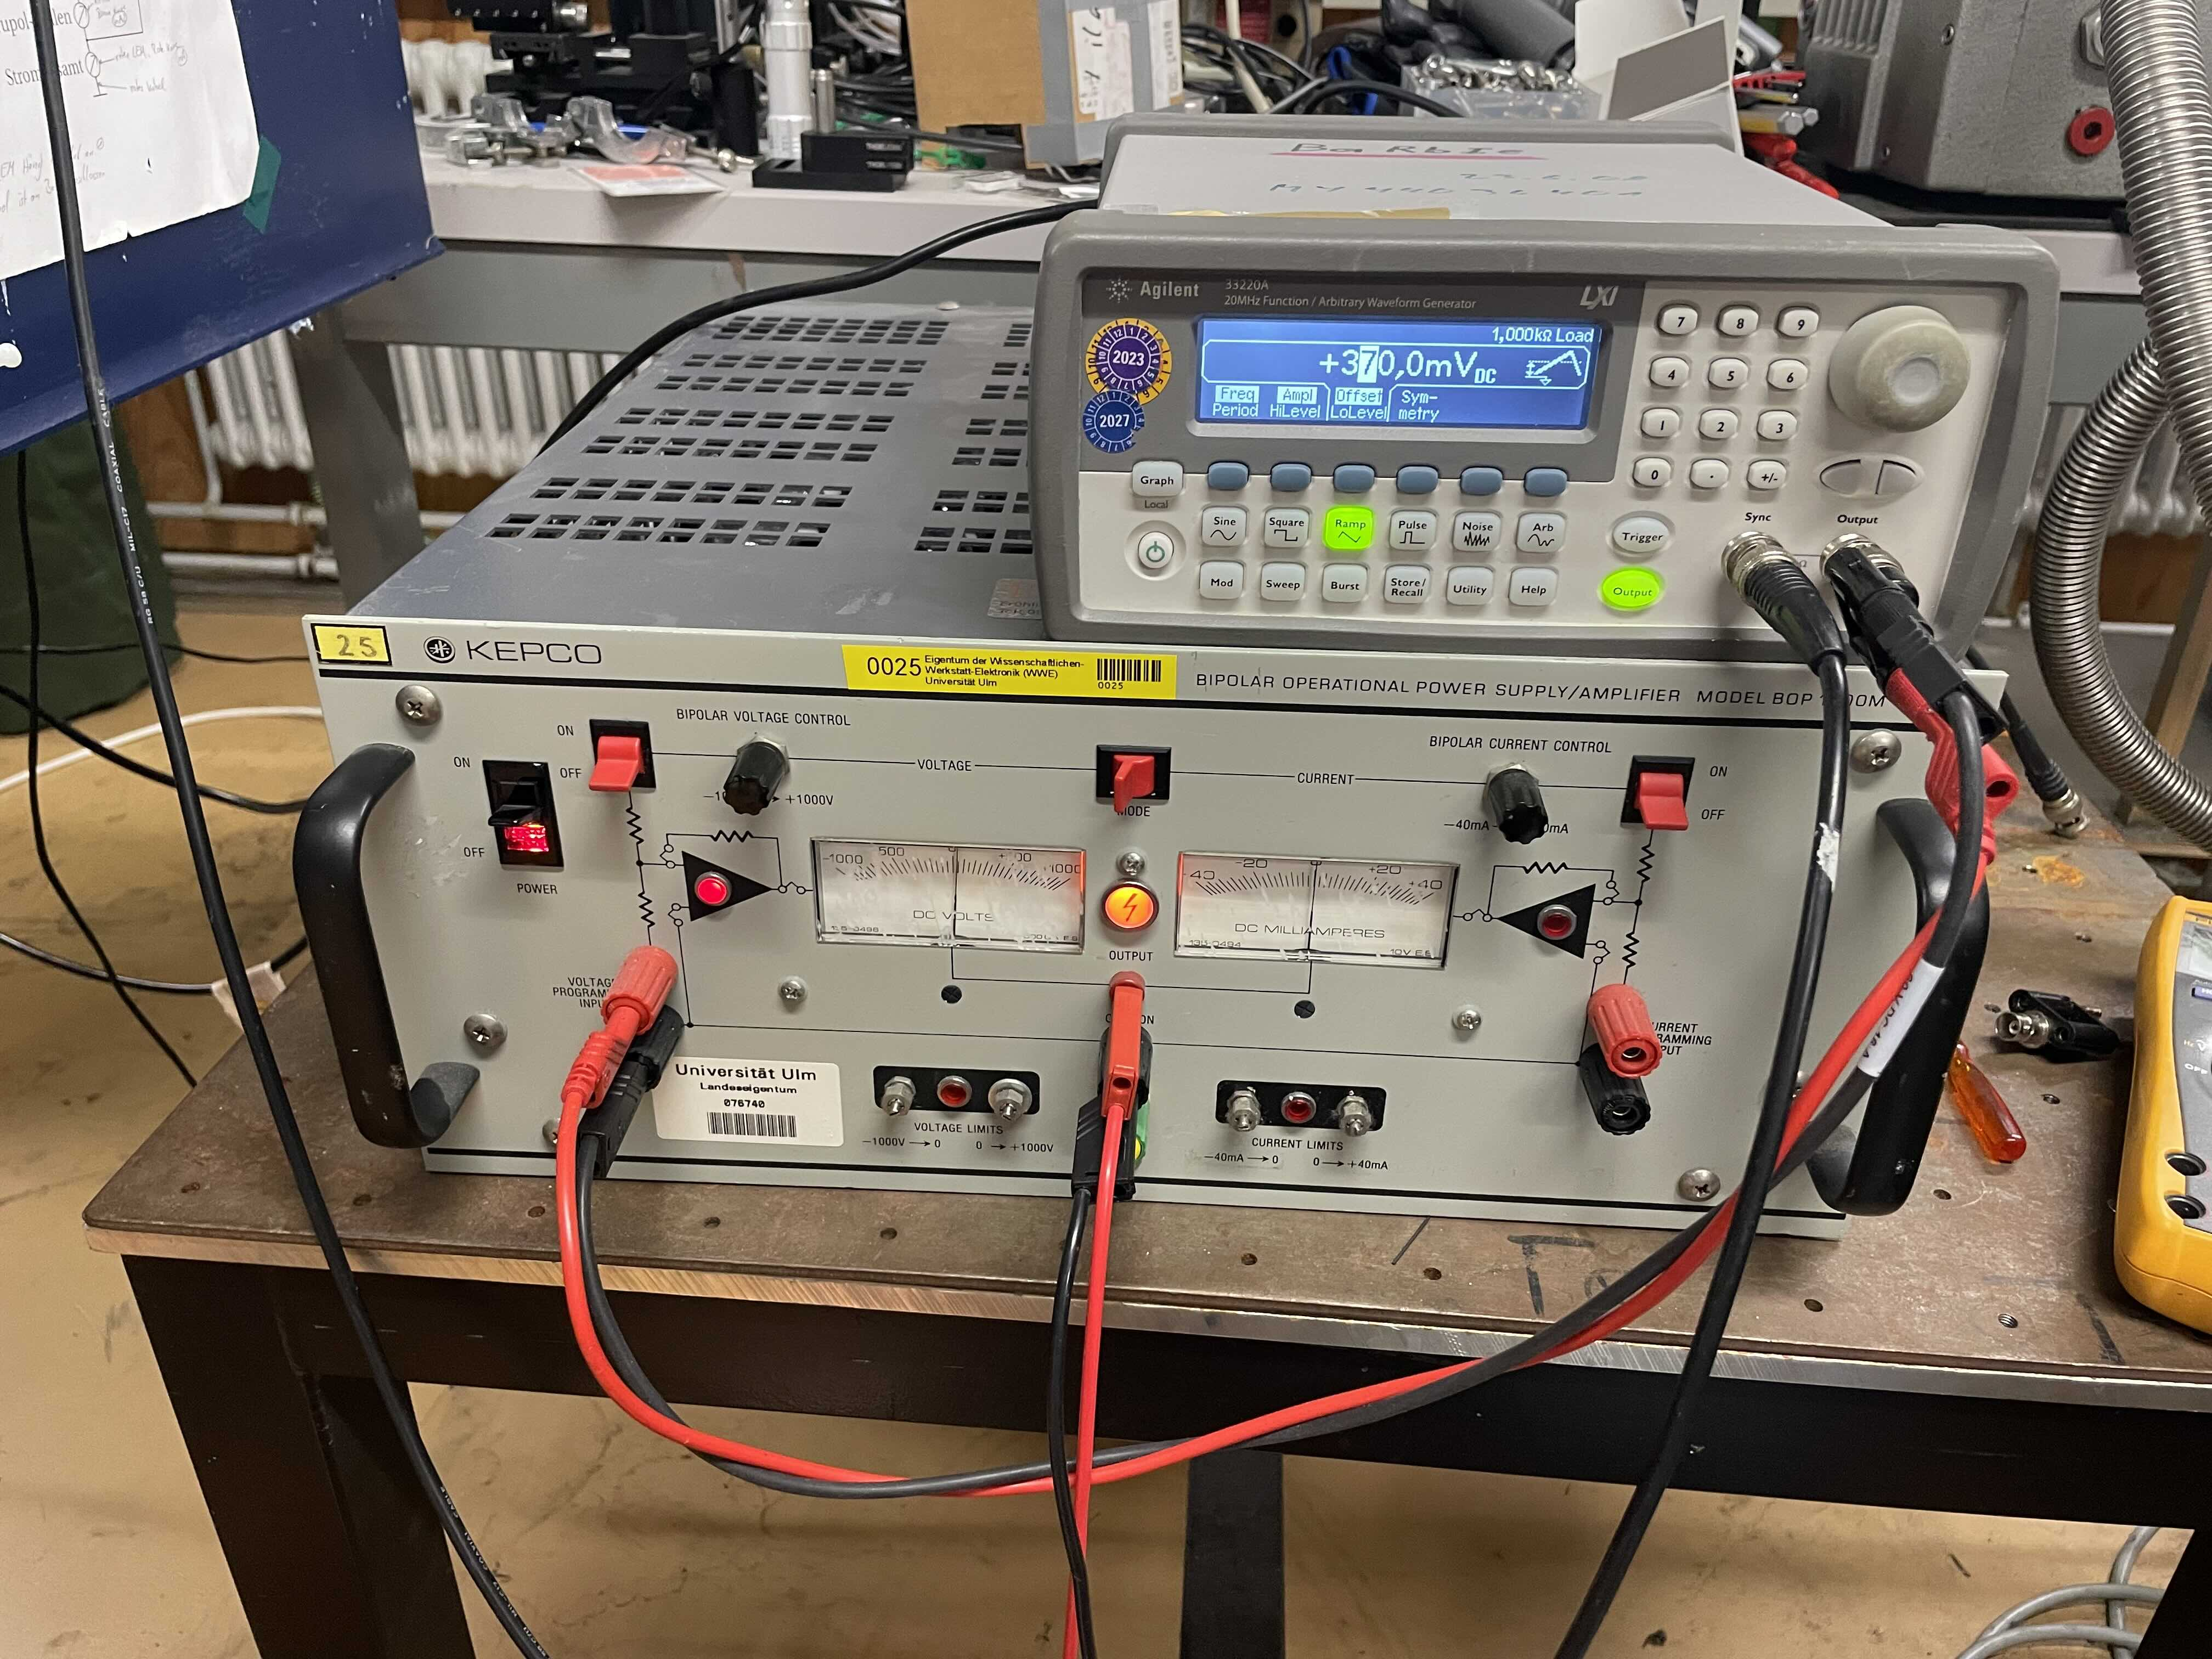
\includegraphics[width=\textwidth]{IMG_8997.jpg}
    \caption{HV Amplifier setup with function generator. Do \textbf{not} exceed the piezo voltage rating. It can only handle $\pm 320$~V at absolute max. We set the limiter light to around 250~V to avoid overshooting.}
\end{figure}

\begin{figure}[htbp]
    \centering
    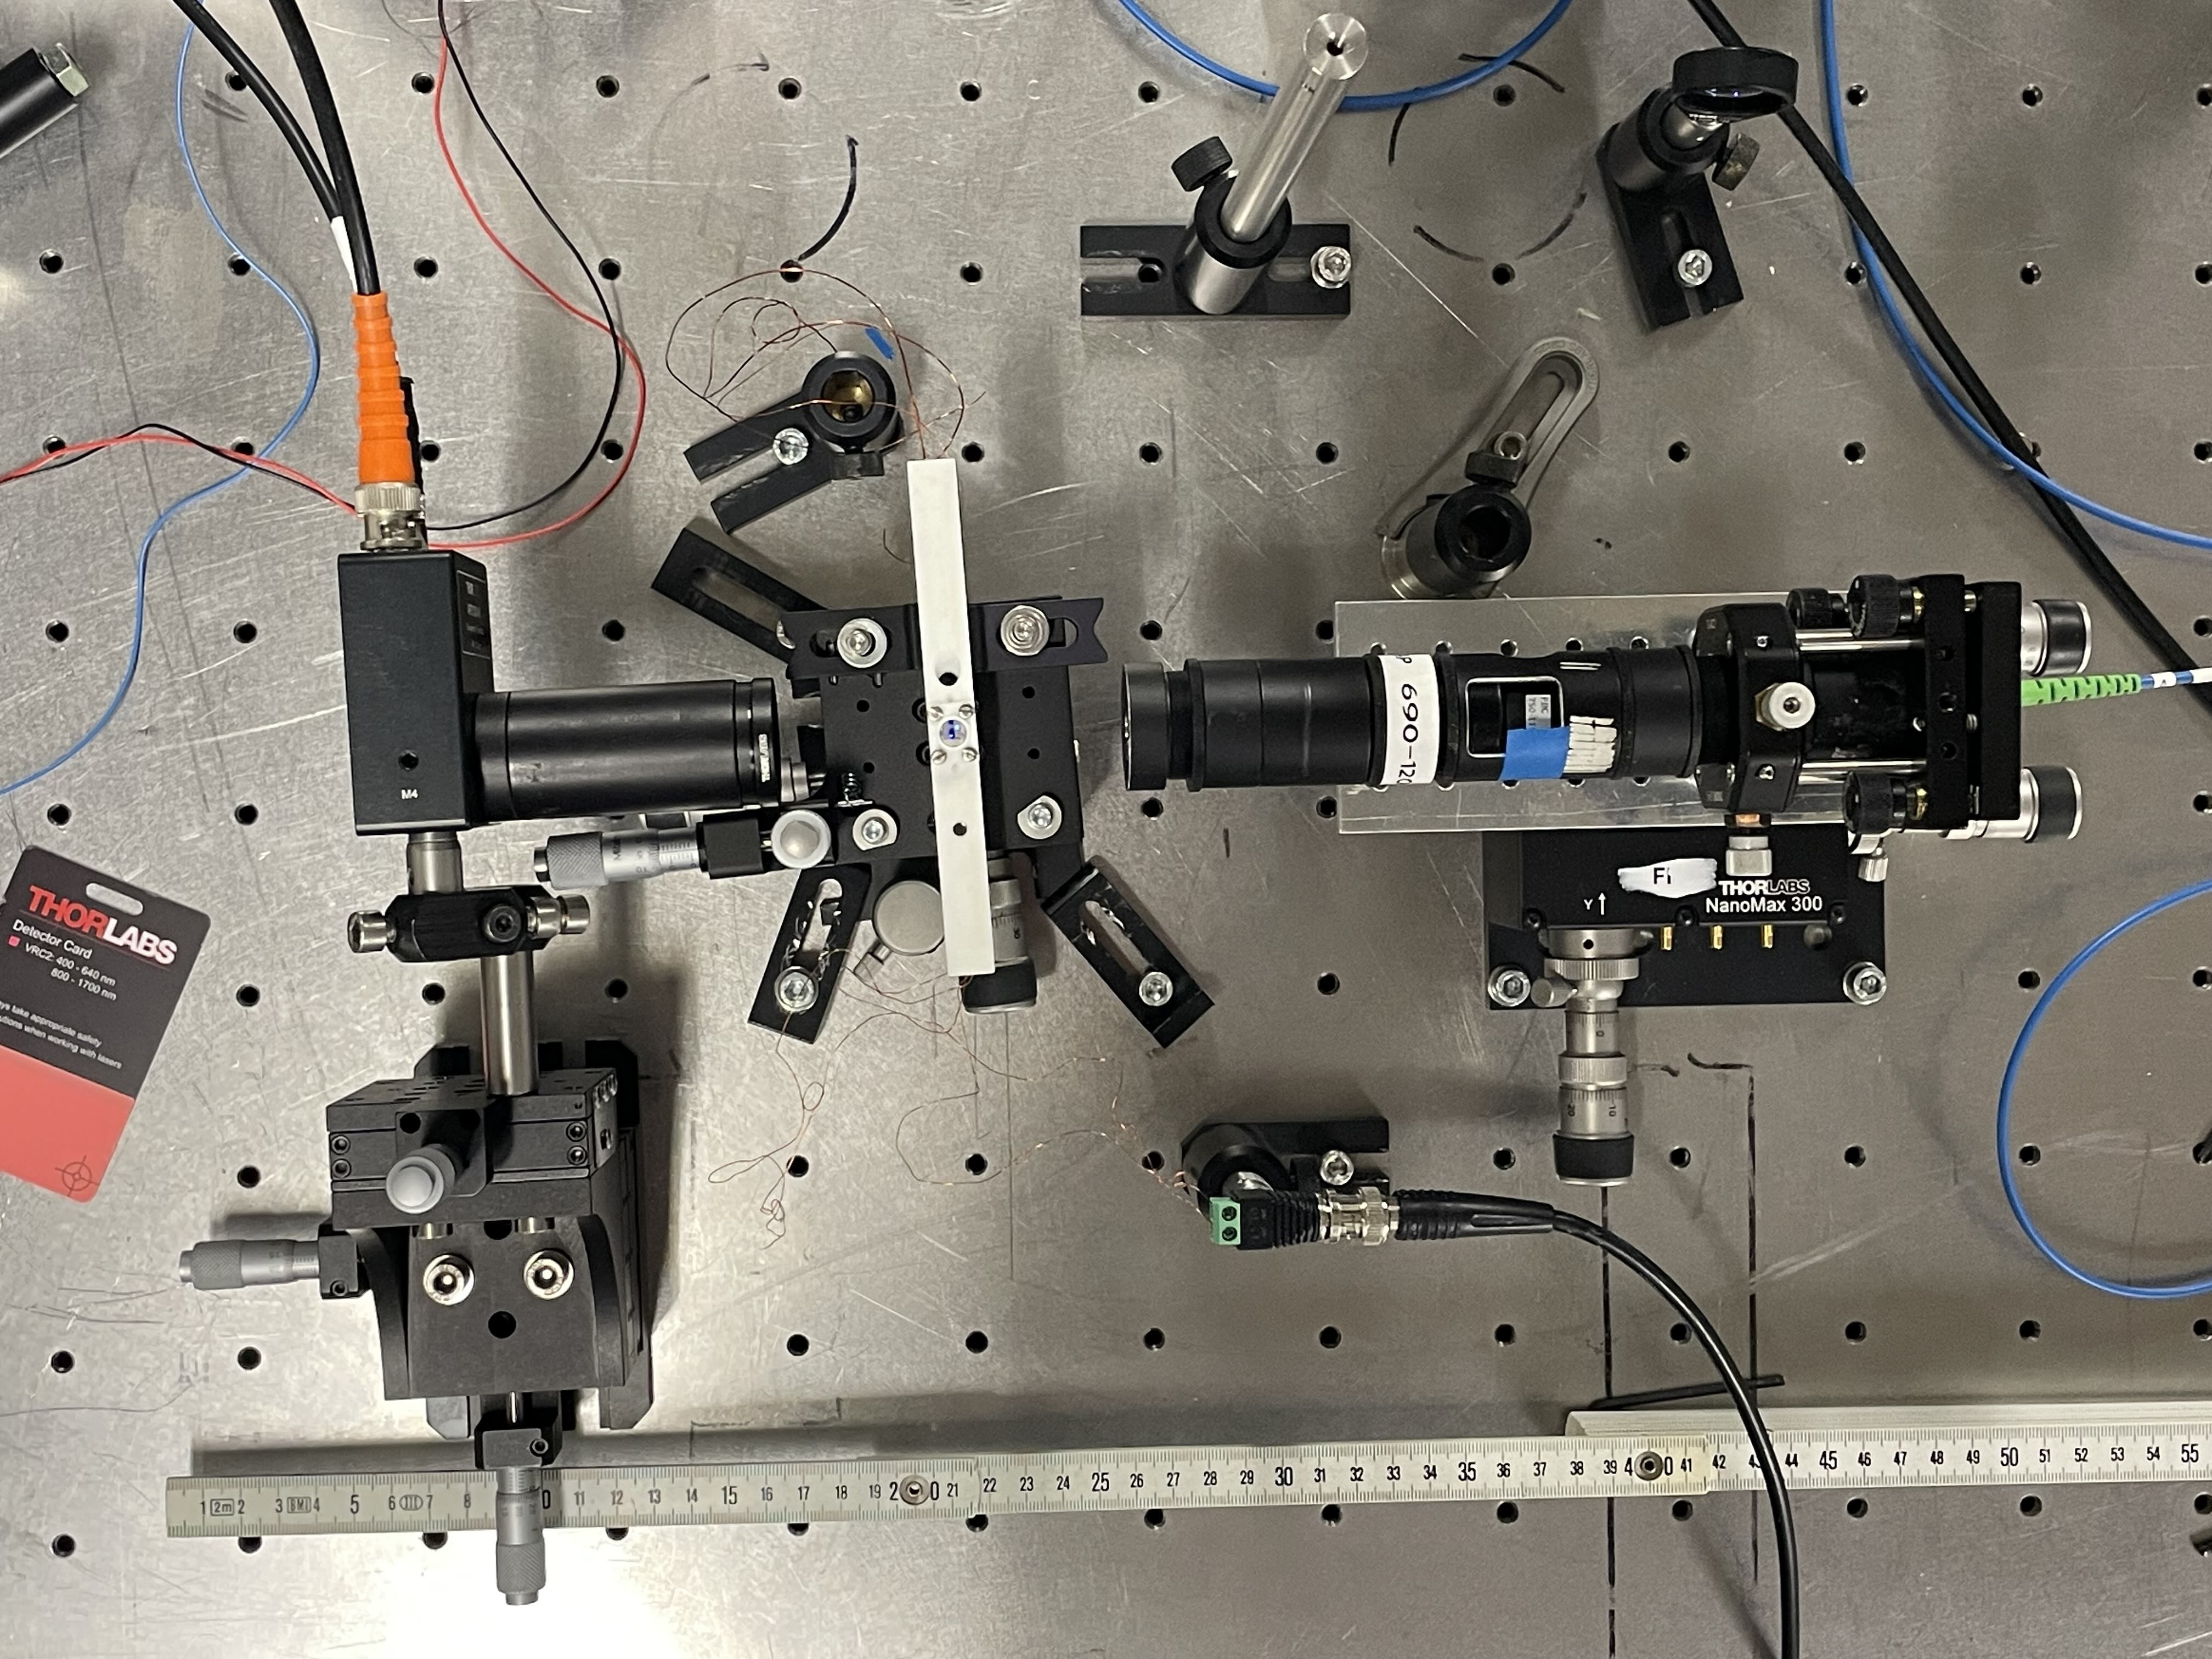
\includegraphics[width=\textwidth]{IMG_8999.jpg}
    \caption{Cavity setup from top view. PD is on the left, incident light is on the right. Incoupling light, cavity and PD are all mounted on individual $xyz$-translation stages. In front of the PD, there is a lens ($f=25.1$~mm) to focus the light onto the sensor.}
    \label{fig:setup}
\end{figure}

\begin{figure}[htbp]
    \centering
    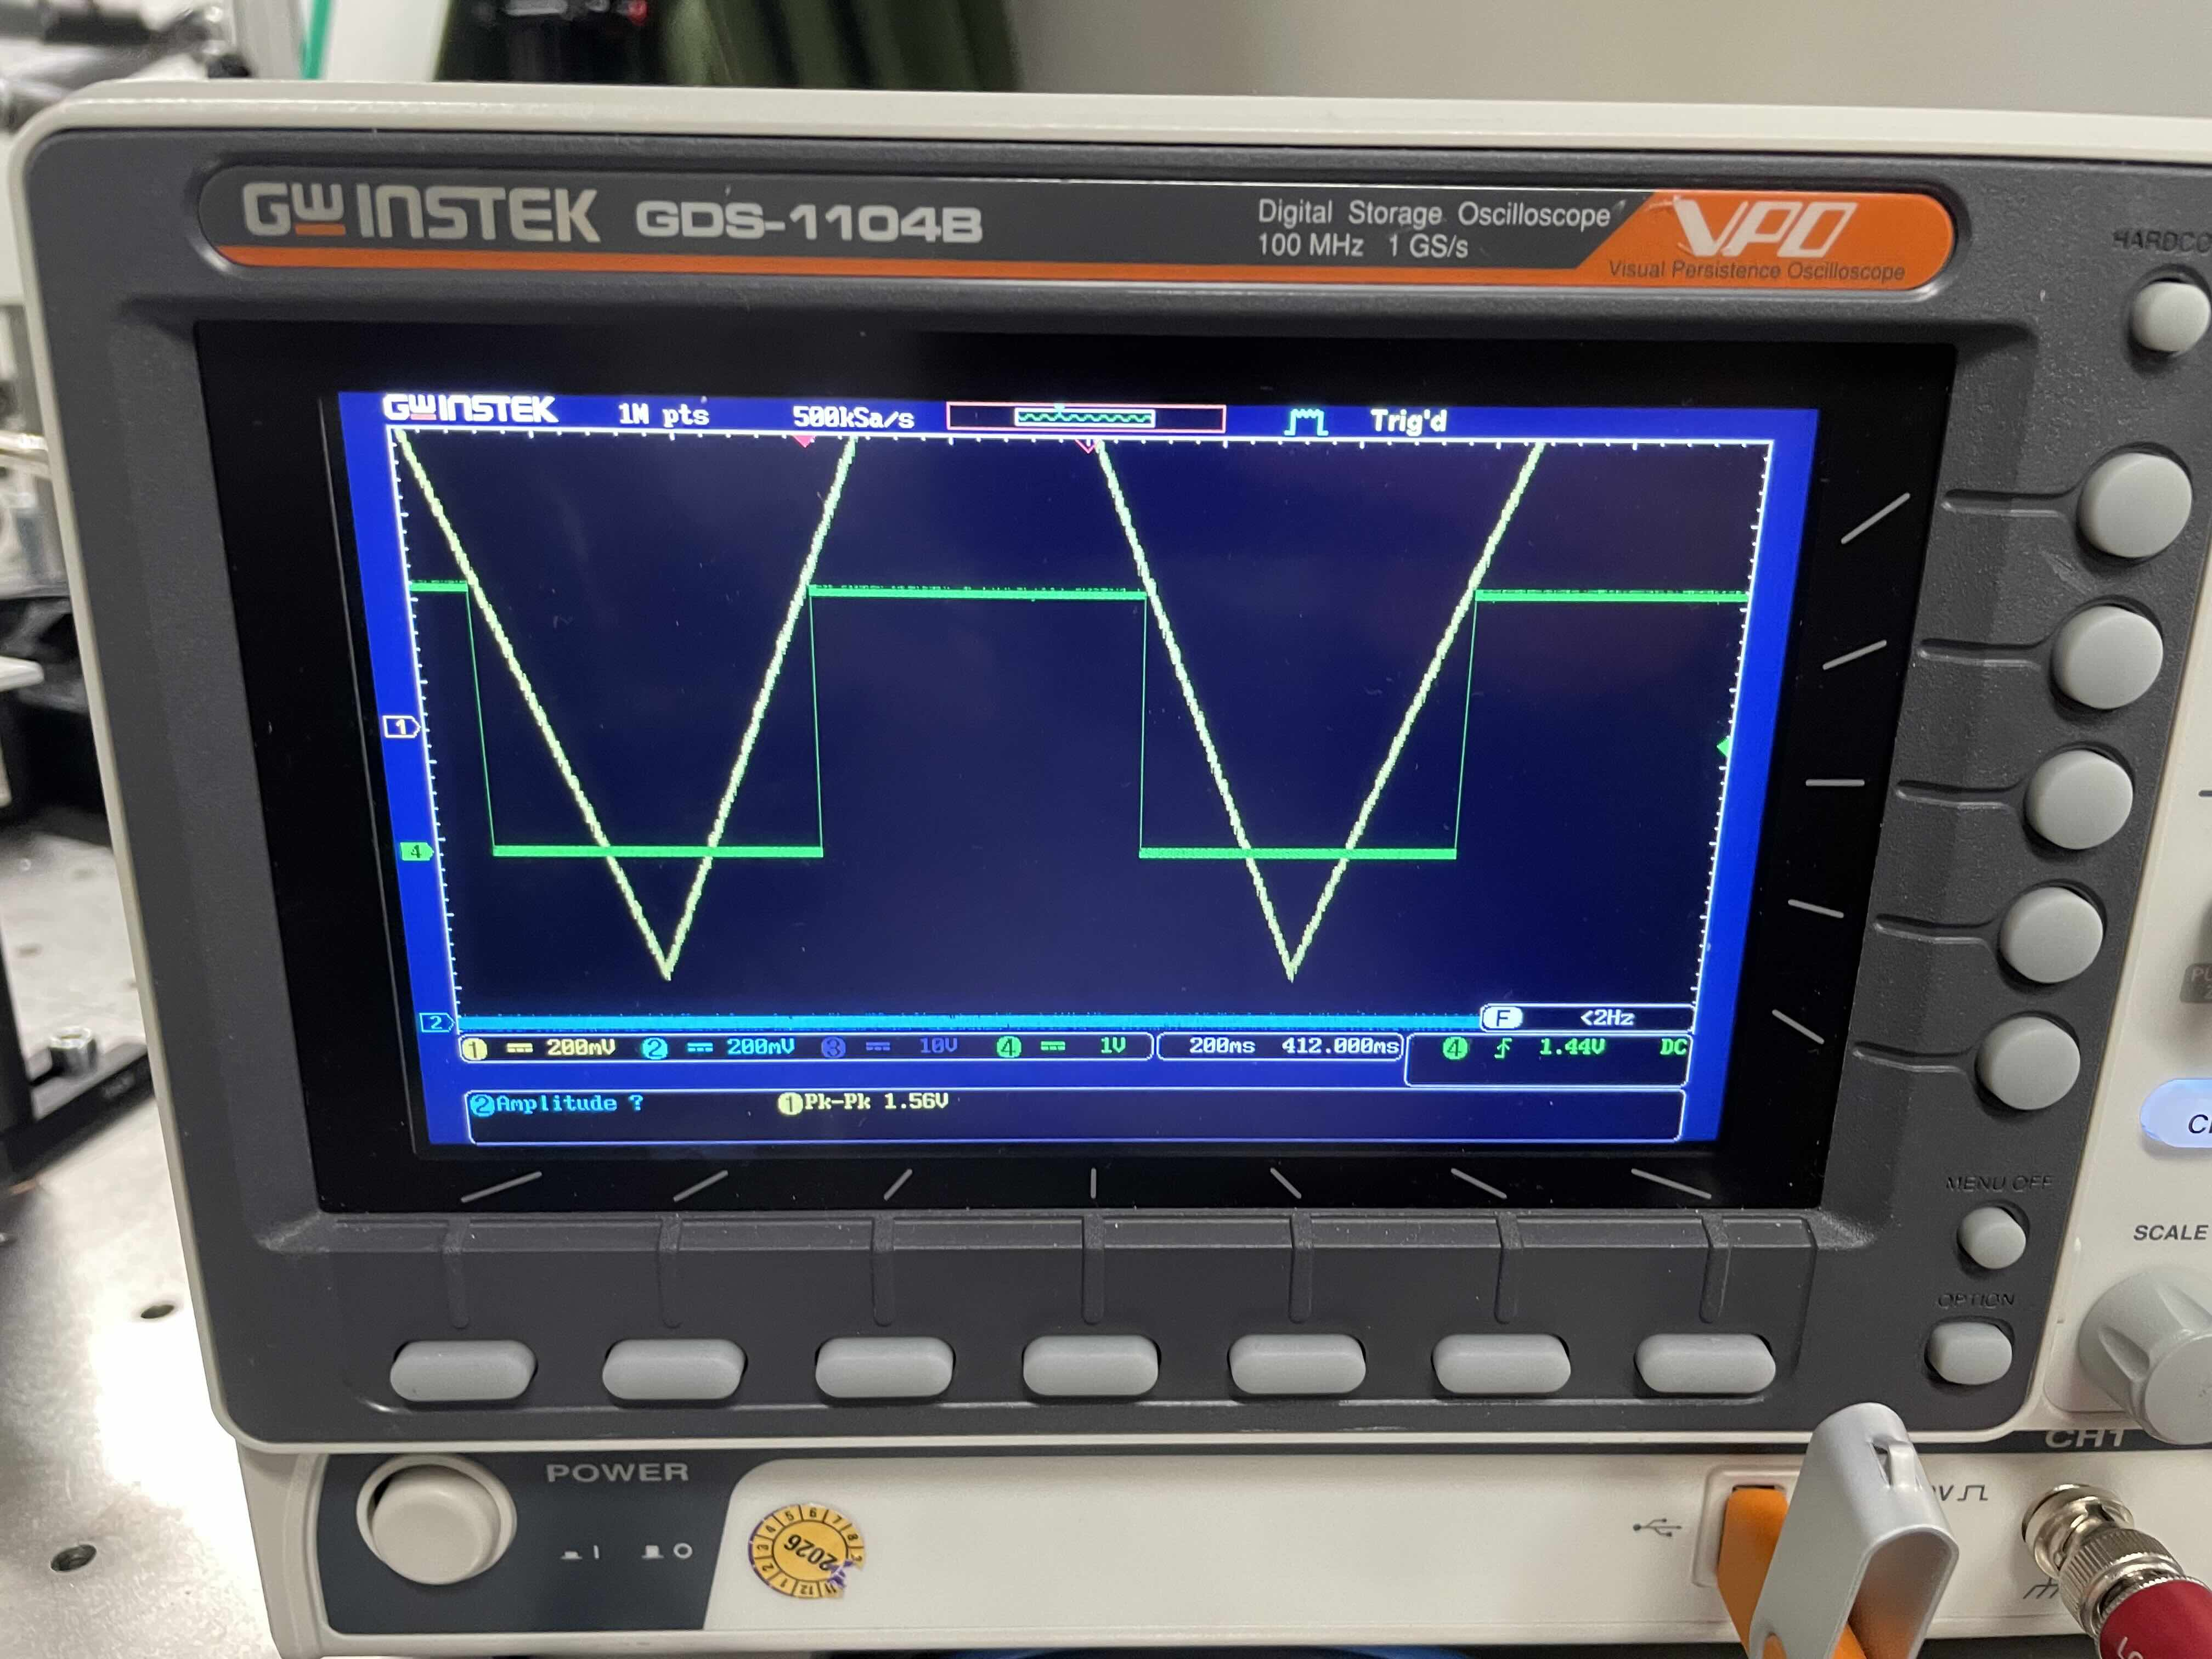
\includegraphics[width=\textwidth]{osci.jpeg}
    \caption{Sync voltage vs piezo driver voltage.}
    \label{fig:osci}
\end{figure}
